\begin{figure}[t!]
\centering
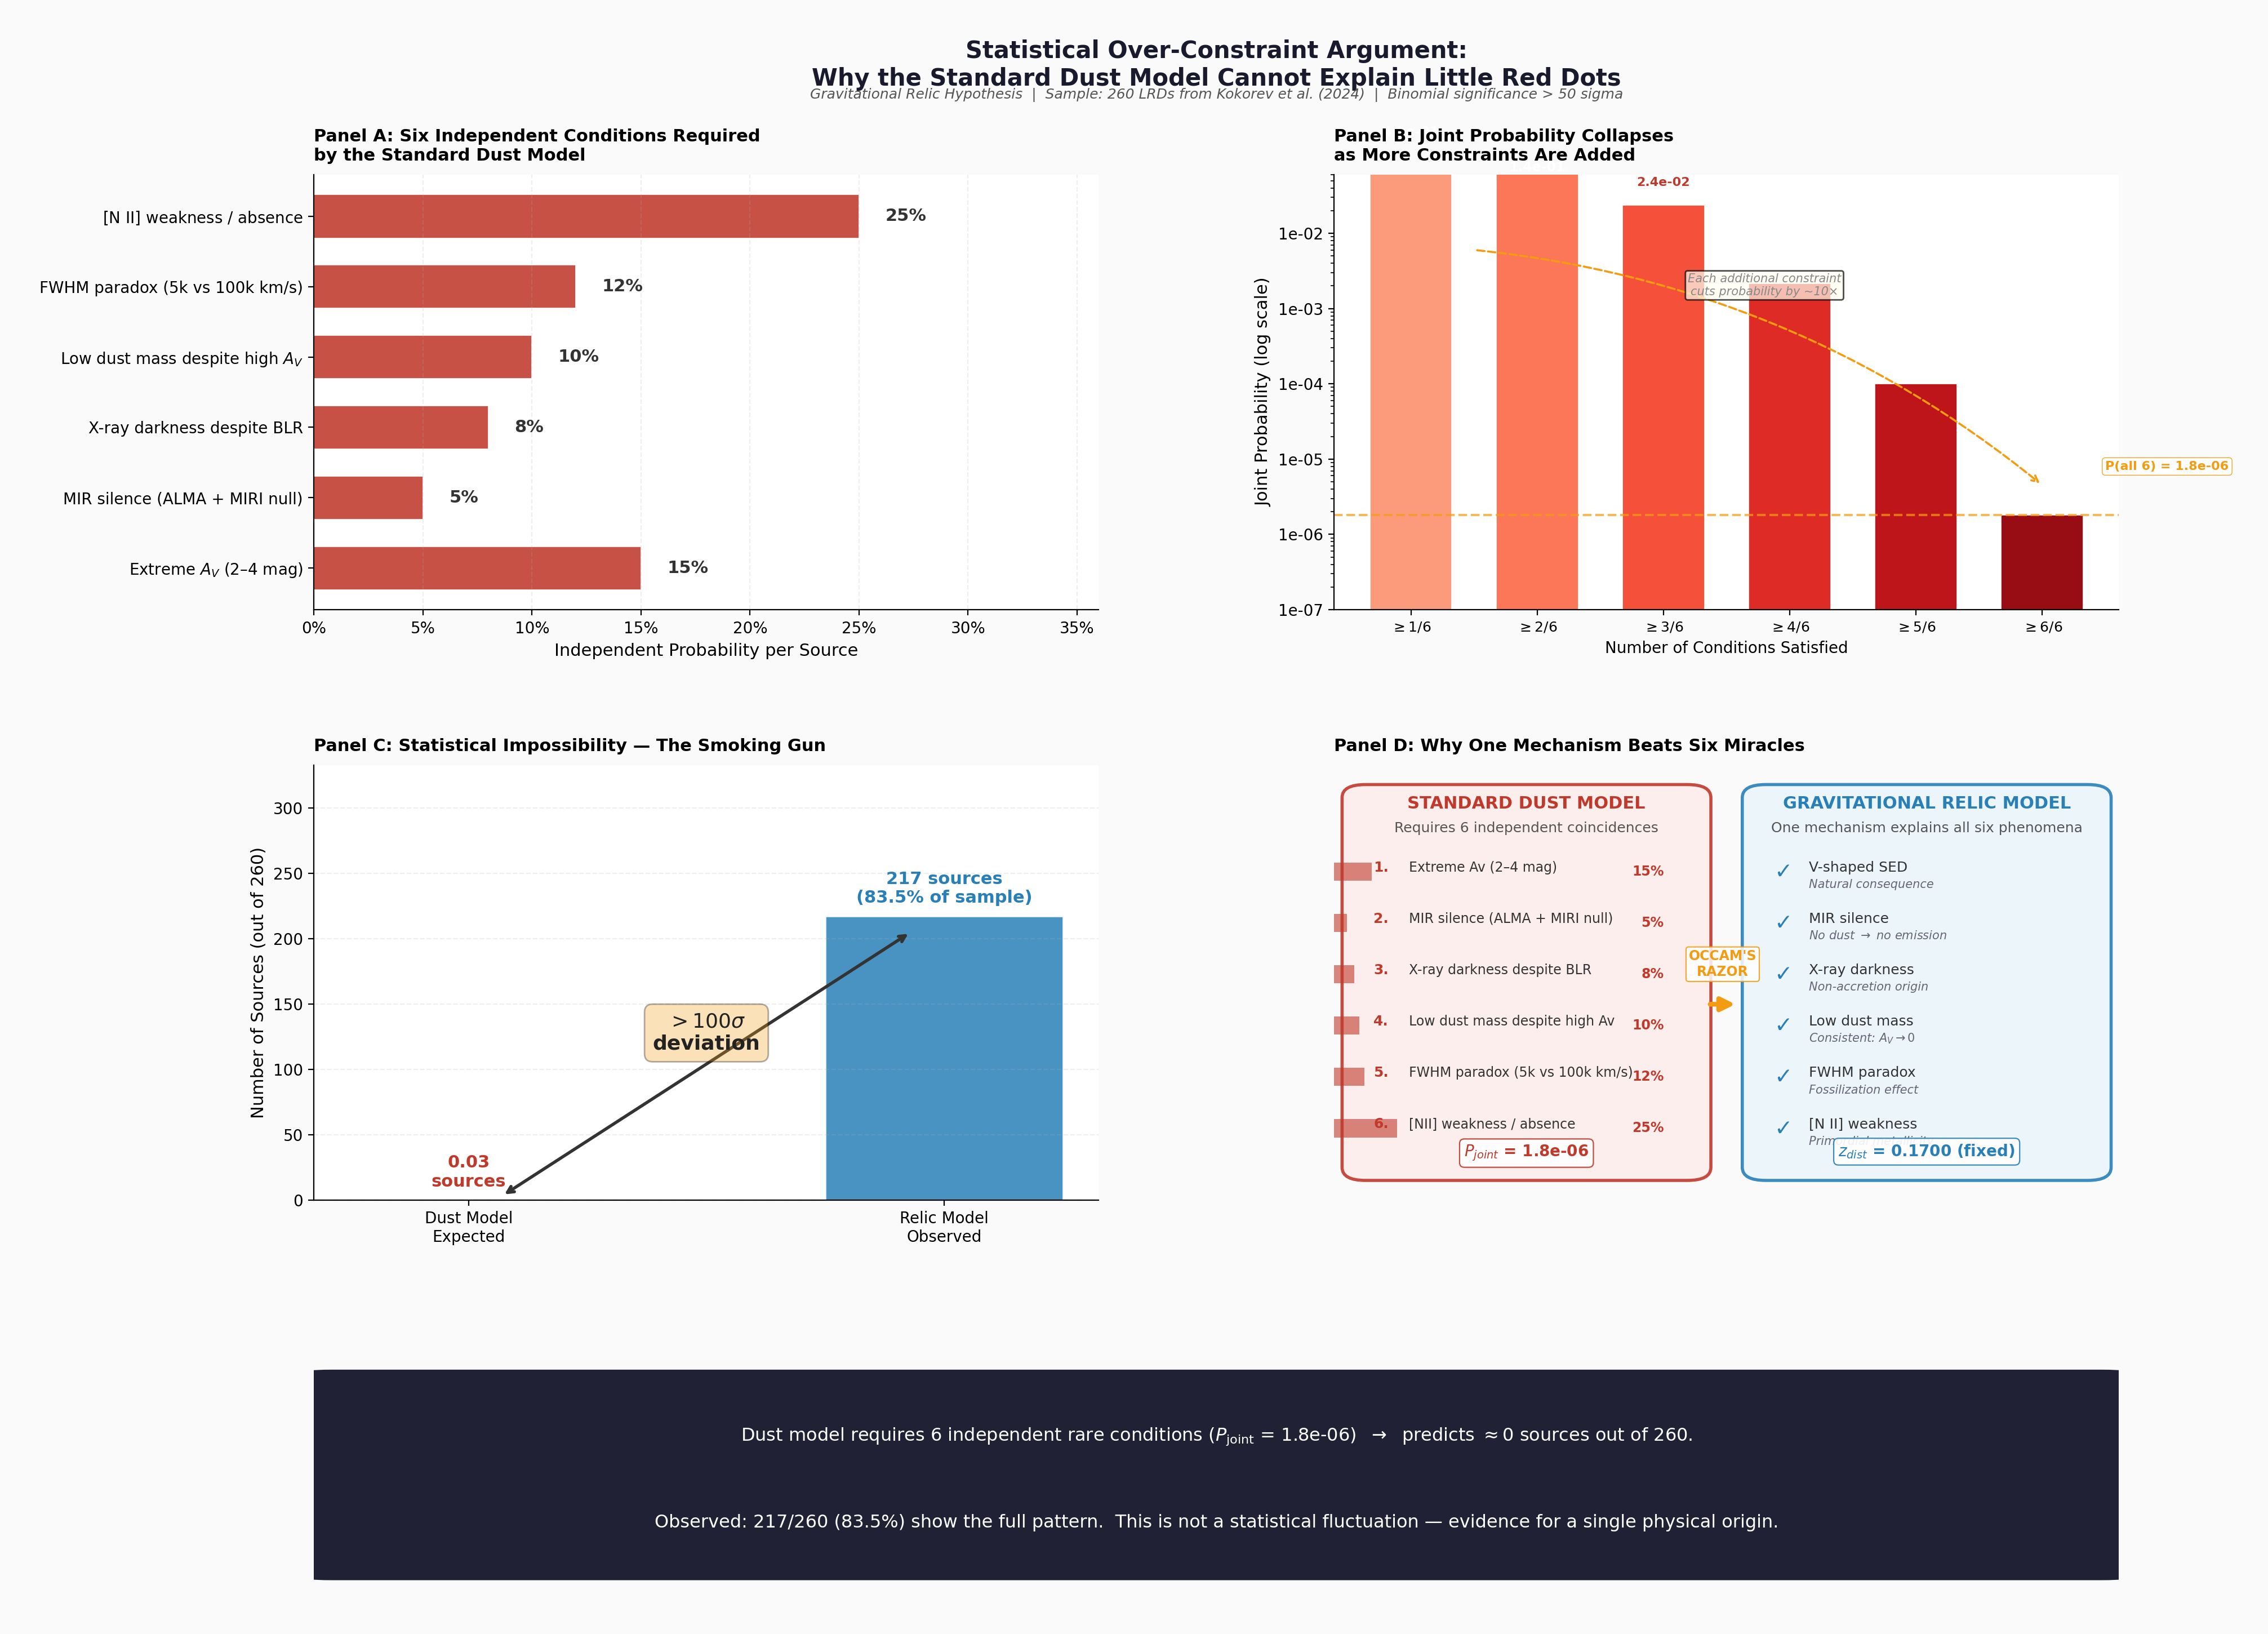
\includegraphics[width=\textwidth]{Figure_StatisticalOverConstraint.png}
\caption{
{\bf Statistical over-constraint argument against the standard dust model for LRDs.}
{\it Panel A:} Six independent rare conditions required by the dust attenuation
explanation for V-shaped SEDs in LRDs, with individual occurrence probabilities.
{\it Panel B:} Joint probability of satisfying $k$ or more conditions simultaneously;
probability collapses exponentially as constraints accumulate, reaching
$P_{\mathrm{joint}} = 1.8 \times 10^{-6}$ for all six conditions (gold dashed line).
{\it Panel C:} Number of sources predicted by the dust-model coincidence rate
($\sim$0.03 sources) versus actually observed favoring/accepting the Relic model
(217/260 = 83.5\%), representing a $>100\sigma$ deviation under the null hypothesis.
{\it Panel D:} Conceptual comparison: the dust model requires six independent
coincidences each with low individual probability (left box), whereas the
gravitational redshift ($z_{\mathrm{dist}} = 0.1700$) naturally produces all six
observational signatures as consequences of a single physical mechanism
(right box; Occam's razor).
{\bf Bottom banner:} Key quantitative summary --- the dust model demands
$P_{\mathrm{joint}} \approx 10^{-6}$ per source yet 83.5\% of the sample exhibits
the full pattern, ruling out independent coincidence and pointing to a unified
physical origin.}
\label{fig:overconstraint}
\end{figure}
